% !TEX encoding = UTF-8 Unicode

\chapter{Introduzione}
L'informatica è il settore tecnologico che si evolve con maggiore velocità. La Prima legge di Moore\footnote{La prima legge di Moore è un'osservazione empirica di Gordon Moore, cofondatore di \emph{Fairchild Semiconductor} e di \emph{Intel}.} asserisce che la potenza dei calcolatori raddoppia ogni diciotto mesi. Una simile progressione in un settore tecnologico assai più anziano come l'aeronautica, permetterebbe oggi di fare un giro completo della terra in una manciata di secondi. Questa potenza di calcolo permette lo sviluppo di applicazioni impensabili fino ad una decina di anni fa, capaci di trattare una quantità di dati da elaborare estremamente grande. Un esempio significativo è l'ammontare di dati che viene generato dai sensori dell'acceleratore di particelle del CERN di Ginevra\footnote{\cite{pres_cern}}, sono circa 15 PetaByte l'anno, i quali devono essere memorizzati e poi elaborati. Il web tutt'oggi genera dati analoghi, ed ogni giorno vengono memorizzati diversi terabyte di dati a seguito di ricerche, acquisti, pubblicazione di contenuti sui social network, eccetera. 
\begin{figure}
	\centering
	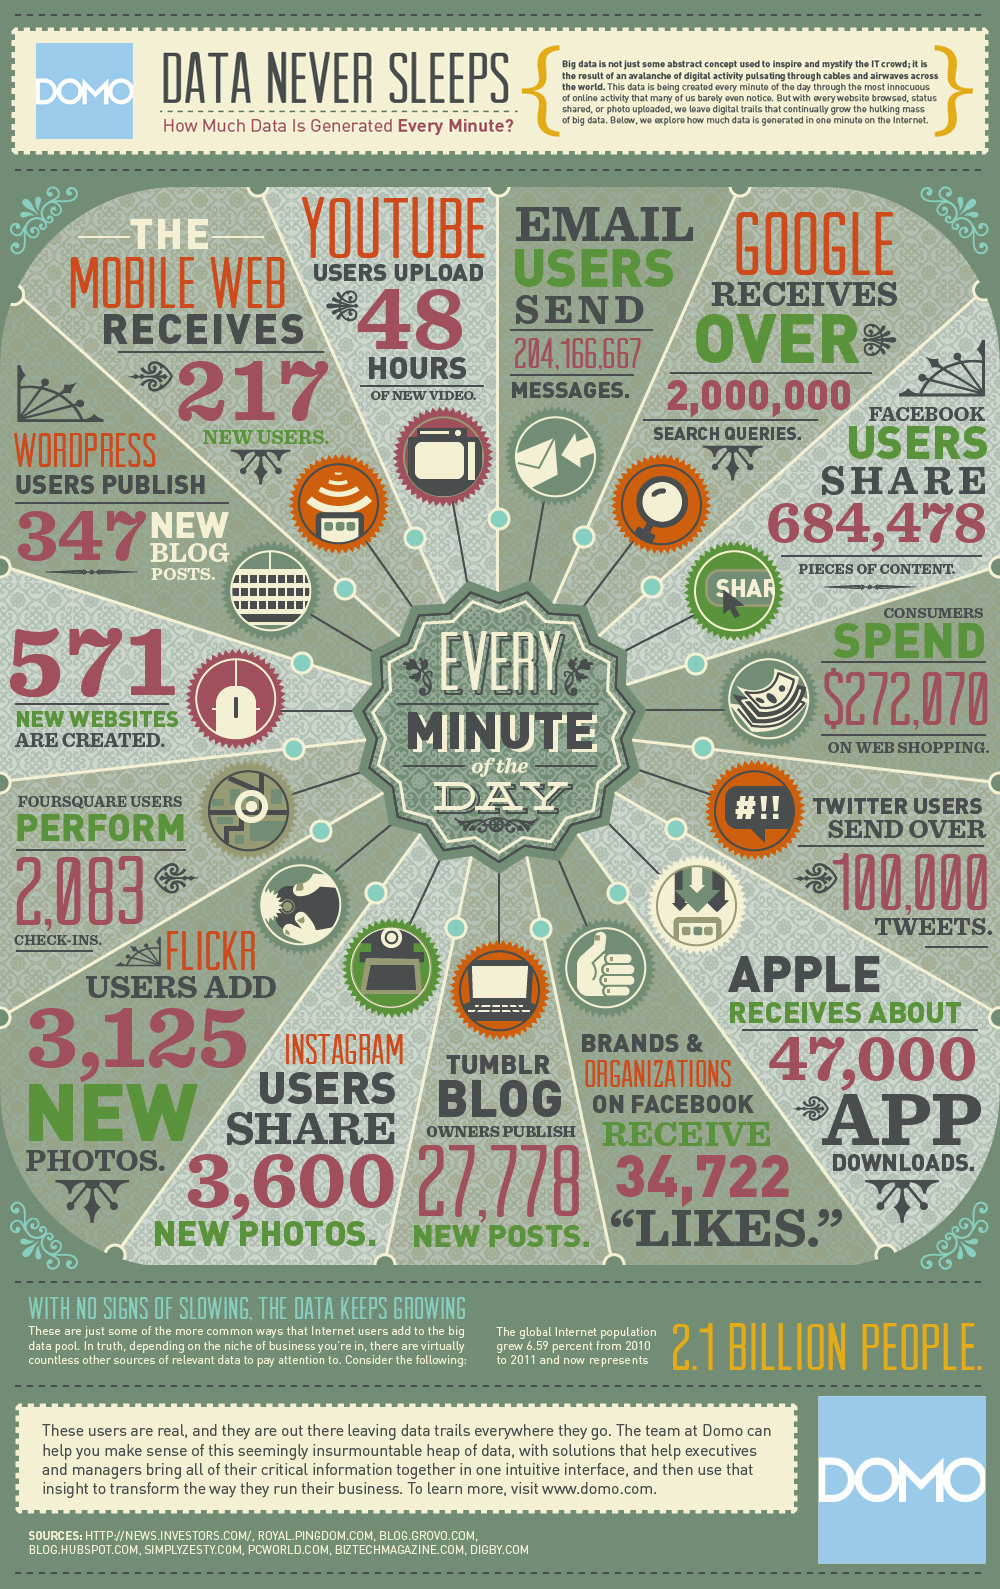
\includegraphics[width=0.50\textwidth]{Data-in-One-Minute.jpg}
	\caption{Quantità di dati al minuto generati dagli utenti di alcuni siti in rete.}
	\label{img:dpm}
\end{figure}
L'infografica nella figura \ref{img:dpm}\footnote{\cite{data_per_minute}} ci permette di vedere con immediatezza di quali quantità stiamo parlando, e possiamo evincere che per una tale mole di informazioni occorrono delle procedure di trattamento dell'informazione diverse da quelle che possono essere adottate da un programma per gestire una semplice rubrica. Stiamo parlando quindi di diversi GigaByte se non TeraByte di dati, che hanno bisogno di essere analizzati e processati in tempo modesto. I tipi di elaborazione necessari possono essere il calcolo di statistiche, una suddivisione per categoria, un'interrogazione della base di dati, oppure una serie di calcoli che possono permettere ad un'azienda di capire, in base agli acquisti dei suoi clienti, i trend riguardo i suoi prodotti. Le tecniche elaborate nel corso degli anni hanno portato alla nascita di una nuova branca dell'informatica, quella dei \emph{Big Data}. Con questo termine non si intendono solo i dataset di grandi dimensioni, ma anche le tecniche utilizzate per \emph{elaborarli} ed estrarre informazioni significative da esso. Spesso non è vero che i dati di un dataset siano omogenei e che tutti rispettino la stessa struttura, perché possono essere il risultato dell'unione di più basi di dati, l'aggiunta di nuovi record può essere effettuata da entità diverse le quali non si preoccupano di seguire una forma standard, per questo motivo è necessario che siano prima \emph{elaborati}. L'\emph{obbiettivo} di queste tecniche è quindi quello di estrarre \emph{informazioni significative}, per le quali intendiamo qualsiasi tipo di statistica che possa essere calcolata solamente prendendo in considerazione tutti i dati esistenti, impossibile da calcolare a mano o farsene un'idea "guardando" i dati. Tornando alla figura \ref{img:dpm}, il risultato dell'elaborazione dei dati è stato presentato in modo da avere un chiaro riscontro, dando la possibilità al lettore di trarre immediatamente le proprie conclusioni sulla globalità dei dati.
Si può suddividere il processo che vede entrare in gioco i big data in tre parti:
\begin{enumerate}
\item Raccolta dei dati
\item Elaborazione
\item Visualizzazione
\end{enumerate}
La raccolta dei dati è la prima parte del processo, e tratta la memorizzazione dei dati ed il loro mantenimento. Non è detto che memorizzazione avvenga su database, ma in qualunque modo, come file di testo o fogli elettronici. Spesso però questa fase è effettuata per altri scopi piuttosto che per effettuare delle elaborazioni tramite gli strumenti dei Big Data. Questo può comportare un dataset formato da dati provenienti da fonti diverse, che utilizzano tecnologie e standard diversi che devono essere aggregati, inoltre non tutti i record potrebbero essere completi, con campi mancanti, dati non consistenti eccetera. Anche questi problemi dovranno essere affrontati.
La parte di elaborazione prevede una serie di tecniche atte ad analizzare tutti i dati in un tempo accettabile, ed effettuare i calcoli. Questa parte prevede anche tutti quegli algoritmi statistici utili ad estrarre informazioni significative da campioni di dati.
La parte di visualizzazione si occupa di presentare i risultati in modo che sia possibile interpretarli immediatamente e farsi un'idea delle proprietà emerse dall'elaborazione rispetto alla totalità dei dati.
In questo testo verranno accennate le prime due parti, mentre per terza parte si presenteranno strumenti di programmazione utili allo scopo, per essere poi applicati al progetto \emph{Piedmont Heritage}.